\documentclass{article}
\usepackage[backend=biber,natbib=true,style=alphabetic,maxbibnames=50]{biblatex}
\addbibresource{/home/nqbh/reference/bib.bib}
\usepackage[utf8]{vietnam}
\usepackage{tocloft}
\renewcommand{\cftsecleader}{\cftdotfill{\cftdotsep}}
\usepackage[colorlinks=true,linkcolor=blue,urlcolor=red,citecolor=magenta]{hyperref}
\usepackage{amsmath,amssymb,amsthm,float,graphicx,mathtools,tikz}
\usetikzlibrary{angles,calc,intersections,matrix,patterns,quotes,shadings}
\allowdisplaybreaks
\newtheorem{assumption}{Assumption}
\newtheorem{baitoan}{}
\newtheorem{cauhoi}{Câu hỏi}
\newtheorem{conjecture}{Conjecture}
\newtheorem{corollary}{Corollary}
\newtheorem{dangtoan}{Dạng toán}
\newtheorem{definition}{Definition}
\newtheorem{dinhly}{Định lý}
\newtheorem{dinhnghia}{Định nghĩa}
\newtheorem{example}{Example}
\newtheorem{ghichu}{Ghi chú}
\newtheorem{hequa}{Hệ quả}
\newtheorem{hypothesis}{Hypothesis}
\newtheorem{lemma}{Lemma}
\newtheorem{luuy}{Lưu ý}
\newtheorem{nhanxet}{Nhận xét}
\newtheorem{notation}{Notation}
\newtheorem{note}{Note}
\newtheorem{principle}{Principle}
\newtheorem{problem}{Problem}
\newtheorem{proposition}{Proposition}
\newtheorem{question}{Question}
\newtheorem{remark}{Remark}
\newtheorem{theorem}{Theorem}
\newtheorem{vidu}{Ví dụ}
\usepackage[left=1cm,right=1cm,top=5mm,bottom=5mm,footskip=4mm]{geometry}
\def\labelitemii{$\circ$}
\DeclareRobustCommand{\divby}{%
	\mathrel{\vbox{\baselineskip.65ex\lineskiplimit0pt\hbox{.}\hbox{.}\hbox{.}}}%
}

\title{Problem: Visual Geometry -- Bài Tập: Hình Học Trực Quan}
\author{Nguyễn Quản Bá Hồng\footnote{A Scientist {\it\&} Creative Artist Wannabe. E-mail: {\tt nguyenquanbahong@gmail.com}. Bến Tre City, Việt Nam.}}
\date{\today}

\begin{document}
\maketitle
\begin{abstract}
	This text is a part of the series {\it Some Topics in Elementary STEM \& Beyond}:
	
	{\sc url}: \url{https://nqbh.github.io/elementary_STEM}.
	
	Latest version:
	\begin{itemize}
		\item {\it Problem: Visual Geometry -- Bài Tập: Hình Học Trực Quan}.
		
		PDF: {\sc url}: \url{https://github.com/NQBH/elementary_STEM_beyond/blob/main/elementary_mathematics/grade_6/visual_geometry/problem/NQBH_visual_geometry_problem.pdf}.
		
		\TeX: {\sc url}: \url{https://github.com/NQBH/elementary_STEM_beyond/blob/main/elementary_mathematics/grade_6/visual_geometry/problem/NQBH_visual_geometry_problem.tex}.
		\item {\it Problem \& Solution: Visual Geometry -- Bài Tập \& Lời Giải: Hình Học Trực Quan}.
		
		PDF: {\sc url}: \url{https://github.com/NQBH/elementary_STEM_beyond/blob/main/elementary_mathematics/grade_6/visual_geometry/problem/NQBH_visual_geometry_solution.pdf}.
		
		\TeX: {\sc url}: \url{https://github.com/NQBH/elementary_STEM_beyond/blob/main/elementary_mathematics/grade_6/visual_geometry/problem/NQBH_visual_geometry_solution.tex}.
	\end{itemize}
\end{abstract}
\tableofcontents

%------------------------------------------------------------------------------%

\section{Equilateral Triangle, Equilateral Hexagon -- Tam Giác Đều, Lục Giác Đều}

\begin{baitoan}[\cite{Binh_boi_duong_Toan_6_tap_1}, H1--H4, p. 69]
	{\rm Đ{\tt/}S?} (a) Tam giác có 3 cạnh bằng nhau là tam giác đều. (b) Tam giác có 3 góc bằng nhau là tam giác đều. (c) Các góc của hình thang cân đều bằng nhau. (d) Trong hình lục giác đều, mỗi đường chéo chính song song với 1 cặp cạnh đối diện.
\end{baitoan}

\begin{baitoan}[\cite{Binh_boi_duong_Toan_6_tap_1}, VD1, p. 70]
	Vẽ $\Delta ABC$ đều cạnh dài {\rm4 cm} bằng thước \& compa.
\end{baitoan}

\begin{baitoan}[\cite{Binh_boi_duong_Toan_6_tap_1}, VD2, p. 70]
	Nếu 1 tam giác có 2 góc bằng $60^\circ$ thì tam giác đó là tam giác đều. Dùng thước kẻ \& êke loại có góc nhọn $60^\circ$ để vẽ 1 tam giác đều có cạnh dài {\rm4 cm}.
\end{baitoan}

\begin{baitoan}[\cite{Binh_boi_duong_Toan_6_tap_1}, VD3, p. 70]
	Có 4 tam giác đều bằng nhau được ghép lại như hình sau. Hỏi $\Delta ABC$ có phải là tam giác đều không?
	\begin{center}
		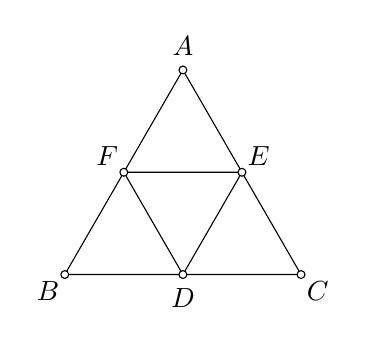
\begin{tikzpicture}
			\path
			(0:0) coordinate (B)
			(0:3) coordinate (C)
			($(B)!1!60:(C)$) coordinate (A)
			($(A)!.5!(B)$) coordinate (F)
			($(B)!.5!(C)$) coordinate (D)
			($(C)!.5!(A)$) coordinate (E);
			\draw (A)--(B)--(C)--cycle (D)--(E)--(F)--cycle;
			\foreach \x/\g in {A/90,B/-135,C/-45,D/-90,E/45,F/135} \draw[fill=white] (\x) circle (.05) + (\g:.3) node{$\x$};
		\end{tikzpicture}
	\end{center}
\end{baitoan}

\begin{baitoan}[\cite{Binh_boi_duong_Toan_6_tap_1}, VD4, p. 71]
	Có 6 tam giác đều giống nhau được ghép lại sao cho chúng có chung 1 đỉnh \& không chồng lên nhau. Hỏi hình tạo thành là hình gì?
\end{baitoan}

\begin{baitoan}[\cite{Binh_boi_duong_Toan_6_tap_1}, VD5, p. 71]
	
\end{baitoan}

\begin{baitoan}[\cite{Binh_boi_duong_Toan_6_tap_1}, VD4, p. 71]
	
\end{baitoan}

\begin{baitoan}[\cite{Binh_boi_duong_Toan_6_tap_1}, VD4, p. 71]
	
\end{baitoan}

\begin{baitoan}[\cite{Tuyen_Toan_6}, 11., p. 78]
	Dùng thước \& compa để vẽ: (a) 1 tam giác đều cạnh {\rm3 cm}. (b) 1 lục giác đều cạnh {\rm2 cm}.
\end{baitoan}

\begin{baitoan}[\cite{Tuyen_Toan_6}, 13., p. 79]
	Cho lục giác đều ABCDEF. Vẽ các đường chéo không phải là đường chéo chính. Kể tên: (a) Các tam giác đều có trong hình. (b) Các hình chữ nhật có trong hình.
\end{baitoan}



\begin{baitoan}[\cite{Tuyen_Toan_6}, 15., p. 79]
	Giải thích vì sao: (a) Có thể dùng 4 viên gạch lát nền hình vuông phủ kín phần nền nhà quanh 1 điểm? (b) Có thể dùng 3 viên gạch lát nền hình lục giác đều phủ kín phần nền nhà quanh 1 điểm? (c${}^\star$) Biết có thể dùng $m$ viên gạch lát nền hình $n$-giác đều phủ kín phần  nhà quanh 1 điểm. Tìm tất cả $n\in\mathbb{N}^\star$ thỏa mãn \& tìm $m$ tương ứng.
\end{baitoan}

%------------------------------------------------------------------------------%

\section{Rectangle, Square -- Hình Chữ Nhật, Hình Vuông}

\begin{baitoan}[\cite{Tuyen_Toan_6}, VD1, p. 75]
	Trong hình sau có bao nhiêu: (a) Hình vuông? (b) Hình chữ nhật?
	\begin{center}
		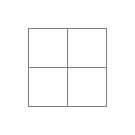
\begin{tikzpicture}[scale=.5]
			\draw[step=1,gray,very thin](0,0) grid (2,2);
		\end{tikzpicture}
	\end{center}	
\end{baitoan}

\begin{baitoan}[\cite{Tuyen_Toan_6}, 1., p. 76]
	Vẽ đoạn thẳng $AB = 4$ {\rm cm} rồi vẽ hình vuông AMBN nhận AB làm 1 đường chéo.
\end{baitoan}

\begin{baitoan}[\cite{Tuyen_Toan_6}, 2., p. 76]
	Vẽ 1 hình vuông lên giấy sau đó cắt hình vuông này thành 4 phần bằng nhau rồi ghép lại thành 2 hình vuông.
\end{baitoan}

\begin{baitoan}[\cite{Tuyen_Toan_6}, 3., p. 76]
	Vẽ đoạn thẳng $AB = 2$ {\rm cm}. (a) Vẽ 2 hình vuông ABCD \& ABEF chung cạnh AB. (b) Tứ giác FDCE là hình gì? Tính các cạnh của FDCE.
\end{baitoan}

\begin{baitoan}[\cite{Tuyen_Toan_6}, 4., p. 76]
	Từ các hình vuông nhỏ cạnh {\rm1 cm}, xếp chúng liền kề nhau thành 1 hình chữ nhật có các cạnh $\ge2$ {\rm cm}. Gọi $n$ là số các hình vuông nhỏ được dùng. Hỏi $n$ là các số nào?
\end{baitoan}

\begin{baitoan}[\cite{Tuyen_Toan_6}, 5., p. 76]
	Vẽ hình theo sự diễn đạt: (a) Vẽ hình chữ nhật ABCD sao cho $CD = 6$ {\rm cm}, $AD = 2$ {\rm cm}. (b) Vẽ hình vuông AMND vào trong hình chữ nhật ABCD. So sánh MN \& BC.
\end{baitoan}

\begin{baitoan}[\cite{Tuyen_Toan_6}, VD4, p. 80]
	Cắt 1 miếng bìa hình vuông thành 4 hình chữ nhật bằng nhau. Biết chu vi mỗi hình chữ nhật là {\rm40 cm}. Tính chu vi hình vuông.
	\begin{center}
		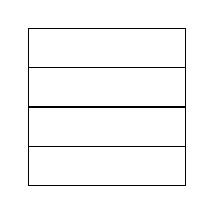
\begin{tikzpicture}[scale=.5]
			\draw
			(0,0) rectangle (4,4)
			(0,1)--(4,1) (0,2)--(4,2) (0,3)--(4,3);
		\end{tikzpicture}
	\end{center}
\end{baitoan}

\begin{baitoan}[\cite{Tuyen_Toan_6}, 16., p. 80]
	Tấm biển hiệu của 1 cửa hàng dài {\rm3 m}, rộng {\rm1 m}. Trang trí viền xung quanh 3 dây đèn {\sc led}. Biết mỗi dây đèn có $125$ bóng đền {\sc led}. Hỏi vòng theo 4 cạnh của tấm biển có bao nhiêu bóng đèn {\sc led}?
\end{baitoan}

\begin{baitoan}[\cite{Tuyen_Toan_6}, 17., p. 80]
	Chiều rộng của 1 hình chữ nhật đúng bằng cạnh của 1 hình vuông. Biết chu vi hình chữ nhật gấp 3 lần chu vi của hình vuông. Hỏi chiều dài của hình chữ nhật gấp mấy lần cạnh hình vuông?
\end{baitoan}

\begin{baitoan}[\cite{Tuyen_Toan_6}, 18., p. 80]
	Hình sau vẽ 1 cánh cửa của tủ bếp. Gỗ làm khung bao quanh có chiều rộng {\rm6 cm}. Phần kính ở giữa rộng {\rm24 cm}, cao {\rm58 cm}. Tính chu vi của cánh cửa này.
	\begin{center}
		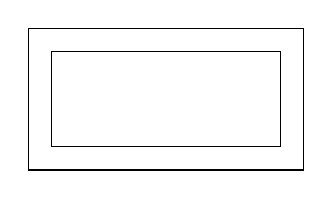
\begin{tikzpicture}[scale=.5]
			\draw
			(0,0) rectangle (7,3.6)
			(0.6,0.6) rectangle (6.4,3);
		\end{tikzpicture}
	\end{center}
\end{baitoan}

\begin{baitoan}[\cite{Tuyen_Toan_6}, 19., p. 80]
	1 miếng bìa hình chữ nhật có chiều rộng là {\rm12 cm}. Ở mỗi góc của tấm bìa, cắt đi 1 hình chữ nhật nhỏ. Phần còn lại là 1 hình có chu vi là {\rm66 cm}. Tính chiều dài ban đầu của tờ bìa.
	\begin{center}
		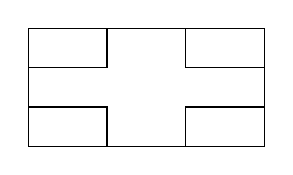
\begin{tikzpicture}[scale=.5]
			\draw
			(0,0) rectangle (6,3)
			(0,0) rectangle (2,1)
			(4,0) rectangle (6,1)
			(0,2) rectangle (2,3)
			(4,2) rectangle (6,3)		;
		\end{tikzpicture}
	\end{center}
\end{baitoan}

\begin{baitoan}[\cite{Tuyen_Toan_6}, 21., p. 82]
	Trồng hoa tại 1 khu đất hình vuông trong công viên. Đường chéo hình vuông là {\rm4 m}. Tính số cây hoa phải trồng biết mỗi $\rm m^2$ trồng $80$ cây hoa.
\end{baitoan}

\begin{baitoan}[\cite{Binh_Toan_6_tap_1}, VD1, p. 101]
	Cho 2 hình vuông có tổng các chu vi bằng {\rm160 cm}. Ghép 2 hình đó lại như hình sau thì hình ghép có chu vi bằng {\rm140 cm}. Tính cạnh của mỗi hình vuông.
	\begin{center}
		\begin{tikzpicture}[scale=.5]
			\draw
			(0,0) rectangle (3,3)
			(1,3) rectangle (2,4);
		\end{tikzpicture}
	\end{center}
\end{baitoan}

\begin{baitoan}[\cite{Binh_Toan_6_tap_1}, VD2, p. 101]
	Tính chu vi 1 hình chữ nhật biết An đo 3 cạnh của hình được {\rm34 cm}, còn Bảo đo 3 cạnh của hình được {\rm32 cm}.
\end{baitoan}

\begin{baitoan}[\cite{Binh_Toan_6_tap_1}, 3., p. 102]
	Cho hình chữ nhật ABCD có $AB = a$, $BC = b$, chu vi $C$. Ở phía ngoài hình chữ nhật đó, vẽ 2 hình vuông ABEG \& BCHK. Gọi $C_1,C_2$ theo thứ tự là chu vi 2 hình chữ nhật CDGE \& ADHK. (a) Biểu thị $C_1,C_2$ theo $C,a,b$. (b) Biết $C_1 = 80$ {\rm cm}, $C_2 = 70$ {\rm cm}. Tính $C,a,b$.
\end{baitoan}

%------------------------------------------------------------------------------%

\section{Parallelogram -- Hình Bình Hành}

\begin{baitoan}[\cite{Tuyen_Toan_6}, VD2., p. 77]
	Có 1 hình bình hành ABCD bằng bìa, cạnh $AB = 5$ {\rm cm}, cạnh $BC = 2$ {\rm cm}. Dùng kéo cắt 1 nhát để được 1 hình bình hành \& 1 hình thoi. Xác định vị trí của nhát cắt.
\end{baitoan}

\begin{baitoan}[\cite{Tuyen_Toan_6}, 6., p. 77]
	Có 2 loại êke: loại êke $60^\circ$ \& loại êke $45^\circ$. Dùng 2 êke bằng nhau để ghép thành: (a) 1 hình chữ nhật. (b) 1 hình bình hành. (c) 1 hình thoi.
\end{baitoan}

\begin{baitoan}[\cite{Tuyen_Toan_6}, 7., p. 77]
	Vẽ hình bình hành ABCD sao cho $AB = 2$ {\rm cm}, $BC = 3$ {\rm cm}, \& $CA = 4$ {\rm cm}.
\end{baitoan}

\begin{baitoan}[\cite{Tuyen_Toan_6}, 20., p. 80]
	Cho hình bình hành ABCD, 2 đường chéo cắt nhau tại O. Cho biết $AC = 2a$, $BD = 2b$, \& tổng chu vi của 4 tam giác đỉnh O là $4a + 4b + 16$. Tính chu vi hình bình hành ABCD.
\end{baitoan}

\begin{baitoan}[\cite{Tuyen_Toan_6}, VD5, p. 81]
	So sánh: (a) Diện tích hình chữ nhật ABCD với diện tích hình bình hành ABDE. (b) Chu vi hình chữ nhật ABCD \& chu vi hình bình hành ABDE biết $AD < AE$.	
	\begin{center}
		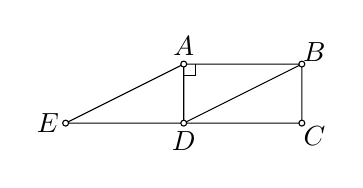
\begin{tikzpicture}[scale=.75]
			\path
			(0,0) coordinate (D)
			(-2,0) coordinate (E)
			(0,1) coordinate (A)
			(2,0) coordinate (C)
			(2,1) coordinate (B)
			;
			\draw (A)--(B)--(C)--(D)--(D)--(E)--cycle (A)--(D) (B)--(D)
			pic[draw, angle radius=1.5mm]{right angle=B--A--D};
			\foreach \x/\g in {A/90,B/45,C/-45,D/-90,E/180} \draw[fill=white] (\x) circle (.05) + (\g:.3) node{$\x$};
		\end{tikzpicture}
	\end{center}
\end{baitoan}

%------------------------------------------------------------------------------%

\section{Rhombus -- Hình Thoi}

\begin{baitoan}[\cite{Tuyen_Toan_6}, 8., p. 77]
	Vẽ hình thoi ABCD sao cho $AC = 6$ {\rm cm} \& $BD = 3$ {\rm cm}.
\end{baitoan}

\begin{baitoan}[\cite{Tuyen_Toan_6}, 9., p. 77]
	Vẽ hình thoi ABCD sao cho độ dài mỗi cạnh là {\rm3 cm} có $\widehat{A} = 50^\circ$.
\end{baitoan}

\begin{baitoan}[\cite{Tuyen_Toan_6}, 10., p. 77]
	Cho 7 điểm $A,B,C,D,E,F,G$. Viết các nhóm 4 điểm trong 7 điểm đó là 4 đỉnh của: (a) 1 hình chữ nhật. (b) 1 hình bình hành nhưng không là hình chữ nhật.
	\begin{center}
		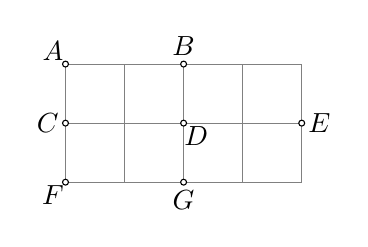
\begin{tikzpicture}[scale=.75]
			\draw[step=1,gray,very thin](0,0) grid (4,2);
			\path
			(0,2) coordinate (A)
			(2,2) coordinate (B)
			(0,1) coordinate (C)
			(2,1) coordinate (D)
			(4,1) coordinate (E)
			(0,0) coordinate (F)
			(2,0) coordinate (G)
			;
			\foreach \x/\g in {A/135,B/90,C/180,D/-45,E/0,F/-135,G/-90} \draw[fill=white] (\x) circle (.05) + (\g:.3) node{$\x$};
		\end{tikzpicture}
	\end{center}
\end{baitoan}

%------------------------------------------------------------------------------%

\section{Isosceles Trapezoid -- Hình Thang Cân}

\begin{baitoan}[\cite{Tuyen_Toan_6}, VD3, p. 78]
	Cho lục giác đều ABCDEF cạnh $a$. Vẽ 3 đường chéo chính. (a) Kể tên tất cả các hình thang cân. (b) Xác định độ dài các cạnh \& số đo các góc của các hình thang cân đó.
\end{baitoan}

\begin{baitoan}[\cite{Tuyen_Toan_6}, 12., p. 78]
	(a) $5$ bậc của 1 cái thang tạo thành mấy hình thang cân? (b) $n$ bậc của 1 cái thang tạo thành mấy hình thang cân?
\end{baitoan}

\begin{baitoan}[\cite{Tuyen_Toan_6}, 14., p. 79]
	Cho hình thang cân ABCD có đáy lớn dài gấp đôi đáy nhỏ. Hỏi: (a) Phải biết độ dài của mấy cạnh thì biết được độ dài của các cạnh còn lại? (b) Phải biết được số đo của mấy góc thì tìm được số đo của các góc còn lại?
\end{baitoan}

%------------------------------------------------------------------------------%

\section{Miscellaneous}

%------------------------------------------------------------------------------%

\printbibliography[heading=bibintoc]

\end{document}